\section{JPA: Object Relational Mapping}

    The technique of bridging the gap between the object model and the relational model is known as object-relational mapping. 
    \begin{definition}
        The challenge of mapping one model to the other lies in the concepts in one model for which there is no logical equivalent in the other is called 
        \emph{impedance mismatch}.
    \end{definition}
    The automatic transformation of a model into another in managed by an element called mediator. The main differences between the object-oriented model and the 
    relational one are the followings: 
    \begin{table}[H]
        \centering
        \begin{tabular}{cc}
        \hline
        \textbf{Object-oriented model}     & \textbf{Relational model}   \\ \hline
        Objects, classes                   & Tables, rows                \\
        Attributes, properties             & Columns                     \\
        Identity (physical memory address) & Primary key                 \\
        Reference to other entity          & Foreign key                 \\
        Inheritance/Polymorphism           & Not supported               \\
        Methods                            & Stored procedures, triggers \\
        Code is portable                   & Not necessarily portable    \\ \hline
        \end{tabular}
    \end{table}
    The Java Persistence API bridges the gap between object-oriented domain models and relational database systems by using a Plain Old Java Object, that is a 
    persistence model for object-relational mapping. 

    The main features of the Java Persistence API are: 
    \begin{itemize}
        \item POJO Persistence: there is nothing special about the objects being persisted, any existing non-final object with a default constructor can be persisted.
        \item Non-intrusiveness: the persistence API exists as a separate layer from the persistent objects.
        \item Object queries: a powerful query framework offers the ability to query across entities and their relationships without having to use concrete foreign keys or database columns.
    \end{itemize}

    \begin{definition}
        The \emph{entity} is a class (Java bean) representing a collection of persistent objects mapped onto a relational table. 

        The \emph{persistence unit} is the set of all classes that are persistently mapped to one database (analogous to the notion of db schema). 

        The \emph{persistence context} is the set of all managed objects of the entities defined in the persistence unit (analogous to the notion of db instance). 

        The \emph{managed entity} is an entity part of a persistence context for which the changes of the state are tracked. 

        The \emph{entity manager} is the interface for interacting with a persistence context. 
        
        The \emph{client} is a component that can interact with a persistence context, indirectly through an entity manager.
    \end{definition}
    The entities are accessed through the entity manager interface of the Java Persistence API. 
    \begin{figure}[H]
        \centering
        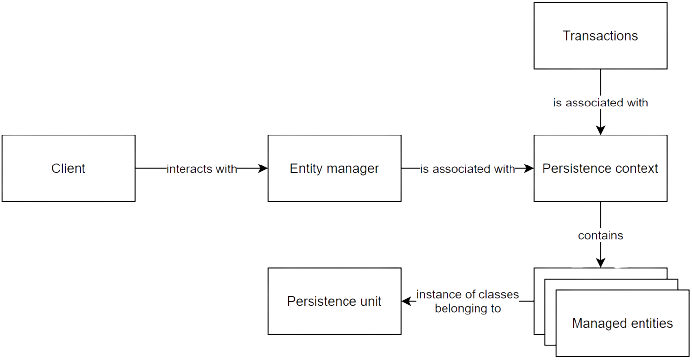
\includegraphics[width=0.6\linewidth]{images/jpa.png}
        \caption{Structure of the Java Persistence API}
    \end{figure}
    The entity manager exposes all the operations needed to synchronize the managed entities in the persistence context to the database to:
    \begin{itemize}
        \item Persist an entity instance in the database.
            \begin{lstlisting}[style=Java]
public void persist(Object entity);
            \end{lstlisting}
        \item Find an entity instance by its primary key.
            \begin{lstlisting}[style=Java]
public <T> T find(Class<T> entityClass, Object primaryKey); 
            \end{lstlisting}
        \item Remove an entity instance from the database.
            \begin{lstlisting}[style=Java]
public void remove(Object entity); 
            \end{lstlisting}
        \item Reset the entity instance from the database.
            \begin{lstlisting}[style=Java]
public void refresh(Object entity); 
            \end{lstlisting}
        \item Write the state of entities to the database immediately.
            \begin{lstlisting}[style=Java]
public void flush();
            \end{lstlisting}
    \end{itemize}
    An entity is a Java Bean that gets associated to a tuple in a database. The persistent counterpart of an entity has a life longer than that of the application. 
    The entity class must be associated with the database table it represents. An entity can enter a managed state, where all the modifications to the object's state
    are tracked and automatically synchronized to the database. The entities have the following properties: identification (primary key), nesting, relationship, 
    referential integrity (foreign key), and inheritance. The entities must respect the following requirements:
    \begin{itemize}
        \item Must have a public or protected constructor with no arguments. 
        \item Must not be final.
        \item No method or persistent instance variables may be final.
        \item Serializable interface must be implemented if you pass the entity by value.
    \end{itemize}
    
    In the database, objects and tuples have an identity (primary key), so an entity assumes the identity of the persistent data it is associated to. The primary key can be 
    either simple or composite. To identify a primary key we use the @Id annotation, for the composite keys we use @EmbeddedId and @IdClass annotations. 
    
    Sometimes, applications do not want to explicitly manage uniqueness of data values. In this case the persistence provider can automatically generate an identifier 
    for every entity instance of a given type. This persistence provider's feature is called identifier generation and is specified by the @GeneratedValue annotation. 
    Applications can choose one of four different ID generation strategy: 
    \begin{enumerate}
        \item Auto. 
        \item Table: identifiers are generated according to a generator table.
        \item Sequence: the identifiers are generated with sequences. 
        \item Identity: the identifiers are generated with primary keys identity columns. 
    \end{enumerate}
    \begin{example}
        An identifier can be generated as follows: 
        \begin{lstlisting}[style=Java]
@Entity
public class Mission implements Serializable {
@Id
@GeneratedValue(strategy = GenerationType.IDENTITY)
private int id;
private String city;
}
        \end{lstlisting}
    \end{example}
    The attributes can be qualified with properties that direct the mapping between POJO and relational tables, such as: 
    \begin{itemize}
        \item Large objects.
        \item Enumerated types: Java enumerations and strings. 
        \item Temporal types.
    \end{itemize}
    The fetch policy can be lazy (retrieve item when needed) or eager (retrieve item as soon as possible). The first policy is used mainly for large objects. 
    \begin{example}
        The qualifiers can be used as follows: 
        \begin{lstlisting}[style=Java]
@Entity
public class Mission implements Serializable {
@Id
@GeneratedValue(strategy = GenerationType.IDENTITY)
private int id;
@Temporal(TemporalType.DATE)
private Date date;
private MissionStatus status;
@Basic(fetch=FetchType.LAZY)
@LOB
private byte[] photo;
}
        \end{lstlisting}
    \end{example}
    By default, entities are mapped to tables with the same name and their fields to columns with the same names, but it is possible to use some annotations 
    to change this behavior. If the entity must be not persistent, we have to denote it with @Transient annotation. 
    \begin{example}
        The mapping can be redefined as follows: 
        \begin{lstlisting}[style=Java]
@Entity @Table(name="T_BOOKS")
public class Book {
@Column(name="BOOK_TITLE", nullable=false)
private String title;
private CoverType coverType;
private Date publicationDate;
@Transient
private BigDecimal discount;
}
        \end{lstlisting}
    \end{example}

    \subsection*{Mapping}
    The relationships in any object model has four characteristics:
    \begin{itemize}
        \item Directionality: each of the two entities may have an attribute that enables access to the other one. If two entities are related with each other we have 
            a bidirectional relationship; otherwise we have a unidirectional relationship. It is possible to have one or more references. 
        \item Role: each entity in the relationship is said to play a role with respect to one direction of access. The entities are classified in source and target,
            based on the direction of the relationship. 
        \item Cardinality: the number of entity instances that exist on each side of the relationship. There are four possibilities: 
            \begin{itemize}
                \item Many-to-one: many source entities, one target entity.
                \item One-to-many: one source entity, many target entities.
                \item One-to-one: one source entity, one target entity.
                \item Many-to-many: many source entities, many target entities.
            \end{itemize}
        \item Ownership: one of the two entity in the relationship is said to own the relationship. In the database, relationships are implemented by a foreign key 
            column (called join column in JPA) that refers to the key of the referenced table. The entities that have  a foreign key column is called the owner of 
            the relationship and its side is called the owning side
    \end{itemize}

    \subsection*{One-to-many relationship}
    The one-to-many bidirectional relationship is defined with mappedBy and @ManyToOne, @OneToMany annotations, where: 
    \begin{itemize}
        \item @ManyToOne annotation to the entity that participates with multiple instances. The entity that contains this annotation is the owner of the relationship. 
        \item @JoinColumn annotation to specify the foreign key column of underlying table. 
    \end{itemize}
    \begin{example}
        First part of the definition of a one-to-many bidirectional mapping. 
        \begin{lstlisting}[style=Java]
@Entity
public class Employee {
@Id private int id;
@ManyToOne
@JoinColumn(name="dept_fk")
private Department dept;
}
        \end{lstlisting}
    \end{example}
    To achieve bi-directionality, the one-to-many mapping direction must be specified too. This is done by including a @OneToMany annotation in the entity that 
    participates with one instance. The @OneToMany annotation is placed on a collection data member and comprises a mappedBy element to indicate the property that 
    implements the inverse of the relationship.
    \begin{example}
        Second part of the definition of a one-to-many bidirectional mapping. 
        \begin{lstlisting}[style=Java]
@Entity
public class Department {
@Id private int id;
@OneToMany(mappedBy="dept")
private Collection<Employee> employees;
}
        \end{lstlisting}
    \end{example}
    Sometimes applications require the access to relationships only along one direction, and in this case the bidirectional mapping is not necessary. 
    
    \subsection*{Many-to-one relationship}
    The many-to-one relationship is defined in the same way as the one-to-many, but the source and the target are switched in the definition. 

    \subsection*{One-to-one relationship}
    To define a one-to-one relationship in JPA it is possible to choose between two different alternatives: 
    \begin{itemize}
        \item We map the relationship as in the bidirectional case and use only the one-to-many direction. 
        \item We do not map the collection attribute in the entity that participates with one instance and use a query instead to retrieve the correlated instances, 
            relying on the inverse (many-to-one) relationship direction mapping.
    \end{itemize}
    The difference between @joincolumn and mappedby is the following: 
    \begin{itemize}
        \item The annotation @JoinColumn indicates the foreign key column that implements the relationship in the database; such annotation is normally inserted in 
            the entity owner of the relationship. Used to drive the generation of the SQL code to extract the correlated instances.
        \item The mappedBy attribute indicates that this side is the inverse of the relationship, and the owner resides in the other related entity. Used to 
            specify bidirectional relationships. In absence of the mappedBy parameter the default JPA mapping uses a bridge table.
    \end{itemize}
    In a one-to-one mapping the owner can be either entity, depending on the database design. A one-to-one mapping is defined by annotating the owner entity 
    with the @OneToOne annotation.
    \begin{example}
        First part of the definition of a one-to-one mapping. 
        \begin{lstlisting}[style=Java]
@Entity
public class Employee {
@Id private int id;
@OneToOne
private ParkingSpace parkingSpace;
}
        \end{lstlisting}
    \end{example}
    If the one-to-one mapping is bidirectional, the inverse side of the relationship needs to be specified too. In the non-owner entity we need both @OneToOne annotation 
    and the mappedBy element (used to JPA to understand where to put the foreign key).
    \begin{example}
    Second part of the definition of a one-to-one mapping. 
        \begin{lstlisting}[style=Java]
@Entity
public class ParkingSpace {
@Id private int id;
@OneToOne(mappedBy="parkingSpace")
private Employee employee;
}
        \end{lstlisting}
    \end{example}

\subsection*{Many-to-many relationship}
    In a many-to-many mapping there is no foreign key column, but there is a join table. Therefore, we can arbitrarily specify as owner either entity.
\begin{example}
    First part of the definition of a many-to-many mapping. 
        \begin{lstlisting}[style=Java]
@Entity
public class Employee {
@Id private int id;
@ManyToMany
private Collection<Project> projects;
}
        \end{lstlisting}
    \end{example}
    If the many-to-many mapping is bidirectional, the inverse side of the relationship needs to be specified too. In the non-owner entity we need both @OneToOne 
    annotation and the mappedBy element.
    \begin{example}
    First part of the definition of a many-to-many mapping. 
        \begin{lstlisting}[style=Java]
@Entity
public class Project {
@Id private int id;
@ManyToMany(mappedBy="projects")
private Collection<Employee> employees;
}
        \end{lstlisting}
    \end{example}
    The logical model of a many-to-many relationship requires a bridge table (join table in JPA). 
    \begin{example}
        The non-default mapping of the entity to the bridge table is specified via annotation. 
        \begin{lstlisting}[style=Java]
@Entity
public class Employee {
@Id private long id;
private String name;
@ManyToMany
@JoinTable(name="EMP_PROJ",
            joinColumns=@JoinColumn(name="EMP_ID"),
            inverseJoinColumns=@JoinColumn(name="PROJ_ID"))
private Collection<Project> projects;
}
        \end{lstlisting}
    \end{example}

\subsection*{Relationship fetch mode}
When the fetch mode is not specified, by default:
\begin{itemize}
    \item A single-valued relationship is fetched eagerly. 
    \item Collection-valued relationships are loaded lazily
\end{itemize}
In case of bidirectional relationships, the fetch mode might be lazy on one side but eager on the other. Note that the best practice is to consider lazy loading 
as the most appropriate mode for all relationships because if an entity as many single-valued relationships that are not all used by applications, the eager mode may 
incur performance penalties. 
\begin{example}
    The annotation used to define the lazy loading.
    \begin{lstlisting}[style=Java]
@Entity
public class Employee {
@Id private int id;
@OneToOne(fetch=FetchType.LAZY)
private ParkingSpace parkingSpace;
}
    \end{lstlisting}
\end{example}
The directive to lazily fetch an attribute is meant only to be a hint to the persistence provider, that can still use an eager policy. The other way round is not true: 
the eager policy cannot be replaced with a lazy one by the provider. 

\subsection*{Cascading operations}
By default, every entity manager operation will not cascade to other entities that have a relationship with the entity that is being operated on. In some cases we want 
to have the propagation of the changes to the entities in relationship with the modified one. It is possible to do so by activating manual cascading. 
\begin{example}
    Activation of manual cascading: 
    \begin{lstlisting}[style=Java]
Employee emp = new Employee();
Address addr = new Address();
emp.setAddress(addr);
em.persist(addr);
em.persist(emp);
    \end{lstlisting}
    With this mode activated, when the entity manager adds the Employee instance to the persistence context, it navigates the address relationship looking for a 
    new Address entity to manage as well. The Address instance must be set on the Employee instance before invoking persist() on the employee object. If an Address 
    instance has been set on the Employee instance and not persisted explicitly or implicitly via cascading, an error occurs.
\end{example}
The cascade attribute is used to define when operations should be automatically cascaded across relationships. It accepts several values: 
\begin{itemize}
    \item Persist. 
    \item Refresh. 
    \item Remove.
    \item Merge.
    \item Detach.
\end{itemize}
If we want to use all the previous operations we can use the operator "all". 
\begin{example}
    Activation of manual cascading of type persist: 
    \begin{lstlisting}[style=Java]
@Entity
public class Employee {
@ManyToOne(cascade=CascadeType.PERSIST)
Address address;
}
    \end{lstlisting}
\end{example}
The cascade settings are unidirectional, so they must be set on both side if we want a bidirectional behavior. 

JPA also supports an additional remove cascading called "orphanRemoval". It is used in @OneToOne and @OneToMany annotations for privately 
owned parent-child relationship in which every child entity is associated only to one parent entity through just one relationship. This operation 
causes the child entity to be removed when the parent-child relationship is broken either by: 
\begin{itemize}
    \item Removing the parent or by setting to null the attribute that holds the related entity. 
    \item In the one-to-many case, by removing the child entity from the parent's collection.
\end{itemize}
The difference between the attribute "CascadeType.REMOVE" and the mode "orphanRemoval" is that if we set manually the value of an entity to null, 
only "orphanRemoval" will automatically remove the linked entities from the database. 